\documentclass{article}
\usepackage{listings}
\usepackage{graphicx} % Required for inserting images
\usepackage{hyperref}
\usepackage[section]{placeins}
\usepackage[utf8]{inputenc}
\usepackage[T1]{fontenc}
 
\usepackage{xcolor}
\title{\underline {\textbf{Summer 2023 Research Summary}}}
\author{Jaehah Shin}
\date{May 15th 2023 ~ TBA}
\begin{document}
\maketitle
\tableofcontents
\section{About the Author}
\quad
My name is Jaehah Shin.
This project is the summer research project that I am currently working on.
I will be second year student this fall in the University of Toronto and I am studying Engineerign Science.
In third year, Engineering Science student will get to choose their major, and I am planning to choose the Robotics major.
I am interested in the field of robotics, and I am planning to study more about the robotics in the future.
I am currently working in the Prof.Franklin's lab in the University of Toronto. 
More information can be found in the following link. \href{https://franklinresearch.ca}{Prof.Franklin's Lab} 
I am currently working on the project that is related to the Induced Local Thermal Hyperemia Coupled with Laser Doppler Flowmetry to Assess Endothelial Function.
The following section will describe the overview of the project that will be worked on this summer. 
\section{Proposal of the Project}
PDF file on the next page is the overview of proposal of the project that I am currently working on.
\begin{figure}[htpb]
    \centering
    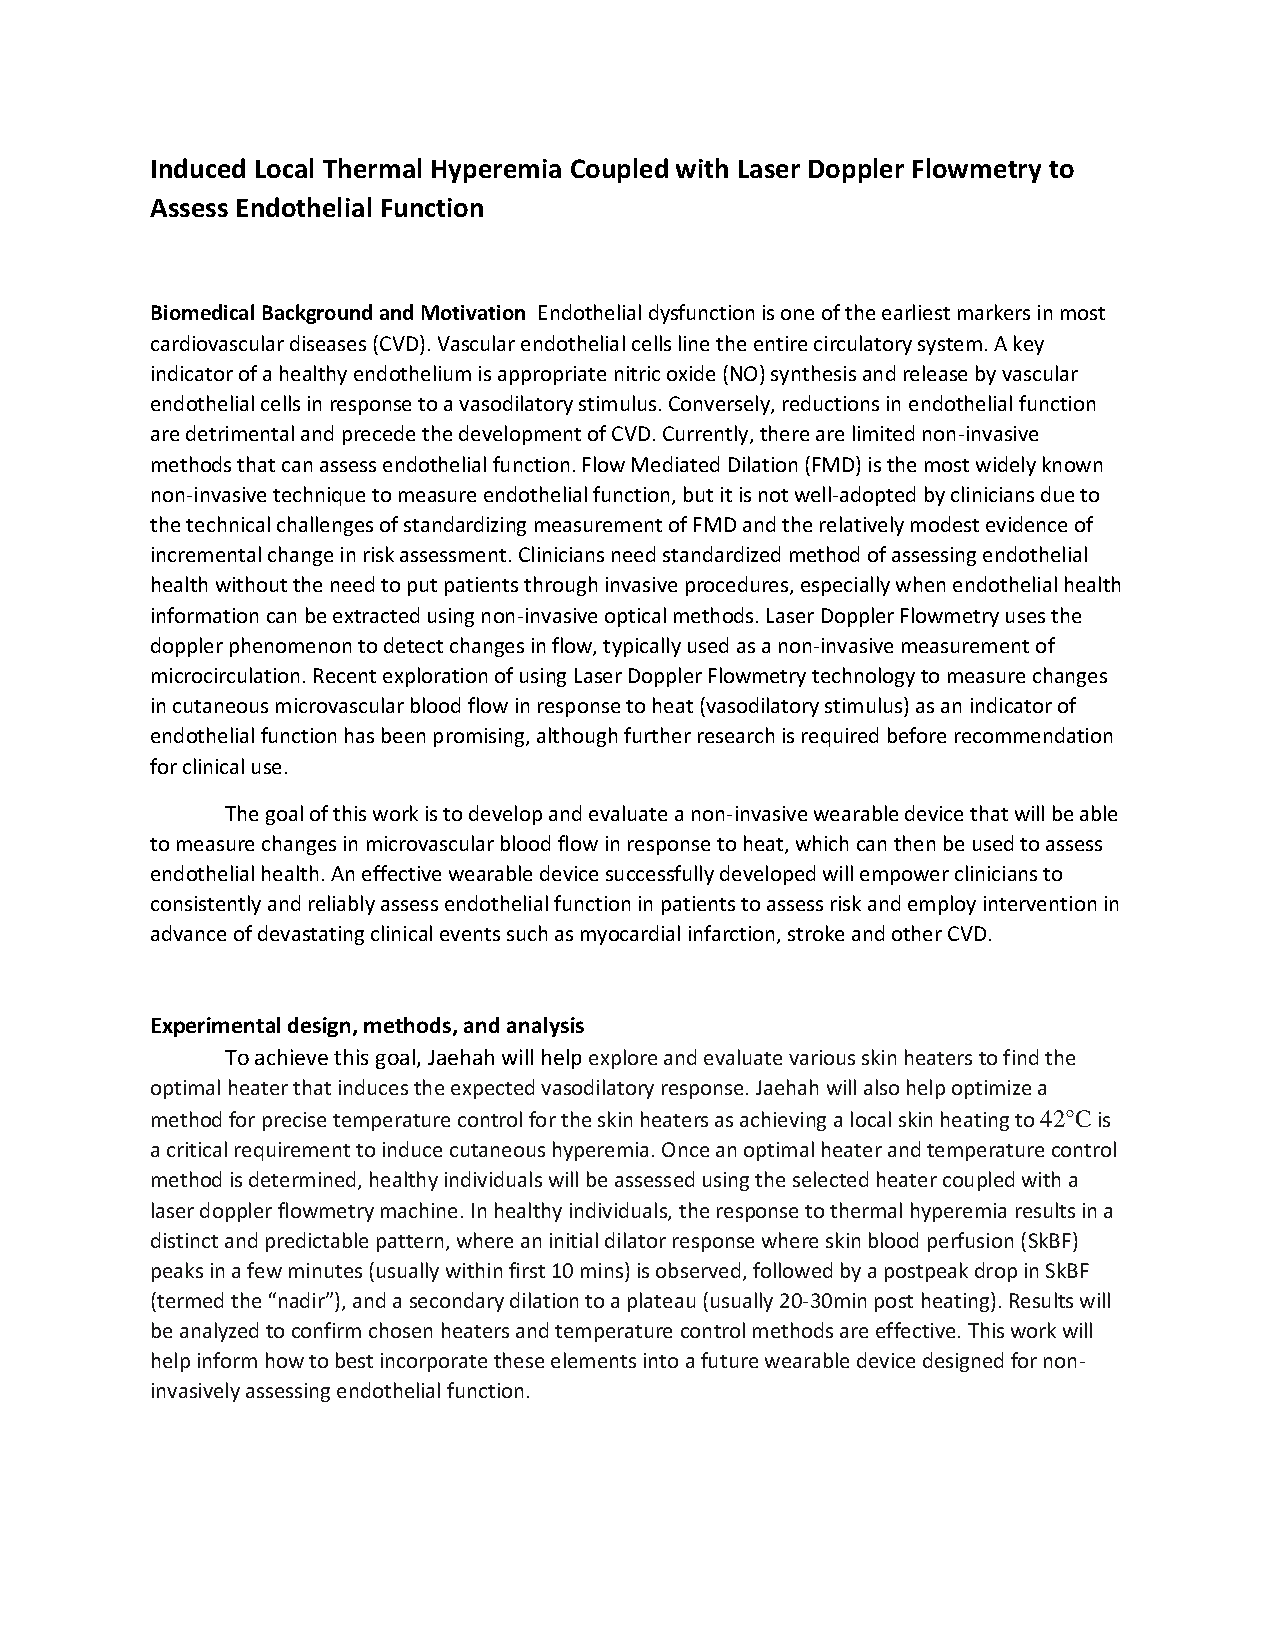
\includegraphics[width=1.1\textwidth]{Jaehah summer research proposal.pdf}
    \caption{The overview of the \texttt{Summer Research Proposal}}
    \label{fig:s_r}
\end{figure}

\section{About the thermister}
On May 15th, my job was to learn about the thermister, and find out how to use this.
Therefore, I did some research about the thermister.

We have all the values for 40.0 degress and 45.0 degrees in the data sheet.
Therefore, we can use datas to cacluate those two temperatures. 
Aim is just to calculate the temperatures in general for lab purposes.

As the resistance of thermister is 10kohm, therefore, resitance of 
wire is negligible.
Thermister doesn't actually read the temperature. 
This reads the resistance of the thermister changes with temperature.

The thermister used in this project is TDK B57230V2103F260 which has 10k ohm.
This is NTC thermister therefore, it has negative temperature coefficient thermistors.
Resistance decreases as temperature rises. 
this is due to the increase in the number of conduction electrons energized by the thermal
agitation from the valance bond. 
Actually, using the termistor is not the best for the accuracy of the temperature.
Since we measure the change of the resistance first and then convert it to the temperature.
Therefore, there are possible errors in the measurement.

However, there is the equation that can calcualte the temperature throuogh the resistance.
Then also the Arduino code can solve that equation. 
That equatino is called as steinhart - Hart equation.

\subsection{Steinhart - Hart Equation}

\LARGE
\begin{equation}
    \frac{1}{T} = A + B\ln(R) + C(\ln(R))^3
\end{equation}
\\
\normalsize
where A, B, C are the constants that are determined by the thermistor and written on the datasheet.
\begin{itemize}
    \item T is the temperature in kelvin
    \item R is the resistance in ohms
    \item A, B, C are the constants that are determined by the thermistor
\end{itemize}

However, there was one big problem with this equation to solve the problem.
On the datasheet provided, there was no A, B, C values.
Therefore, there was only one way to solve this equations which is measuring the resistance at 
three fixed different temeperature. 
As there are three unknowns, we need three equations to solve for A, B, C.
For example, at 40.0 degrees, 45.0 degrees, and 50.0 degrees, we can measure the resistance.

And then compute the values to calculate for A, B, C, then
implement that equation with all the coefficients in the arduino code. 
However, as the lab bought the heater temperature controller, this method is not necessary anymore.
As the heater temperature controller has the thermister, it can read the temperature directly which is 
more accurate than the method that we were planning to use. 

\section{Heater Temperature Controller}
Lab bought the TC300 - Heater Temperature Controller from Thorlabs on May 18th.
\href{https://www.thorlabs.com/drawings/1a9e0ae31580f35c-5554A647-C109-6112-A4FC47A27614B988/TC300-Manual.pdf}{Document on Heater Temperature Controller}
Following paragraph will be the sumamrized note for heater temperature controller on how to use it. 
Thefore, this part will be written based on that doucment.

First, as you can see from below figure, heater can be connected to heater temperature controller.
There is a space that wire can be connected, therefore, connect heater into hole 1 and 2.
\begin{figure}[htpb]
    \centering
    \includegraphics[width=1.1\textwidth]{heater connection.png}
    \caption{The overview of the \texttt{Heater Temperature Controller}}
    \label{fig:s_r}
\end{figure}

Second, connect the thermister to the hole 4 and 5. As you can see from figure below, thermister also can be connected to this device. 
\begin{figure}[htpb]
    \centering
    \includegraphics[width=1.1\textwidth]{Thermister connection.png}
    \caption{The overview of the \texttt{Heater Temperature Controller}}
    \label{fig:s_r}
\end{figure}

Eventhough, there are more featuers in this device, we will focus on the temperature control feature mostly,
therefore, thermister and heater will be connected to this device. 

\subsection{How to use the Heater Temperature Controller}
After, connecting the heater and thermister to the device, this is ready to be used. \\

1. Conenct the powr line to the AC inlet on the back panel with the included power cord. \\
2. Press the rocker switch on the front panel to turn on the device. \\
3. Wait for the device to be initialized, then it will enter home screen.

However, there is \textcolor{red}{Warning} that we need to be careful about.

\textbf{\textcolor{red}{WARNING} : HIGH VOLTAGE INSIDE.} \\
To avoid electrical shock, the power cord protectivee groudning conductor must be connected to the ground.
Without cover installed, the device must not be operated. 

\subsection{Front Panel Operation}
Below is the figure of the front panel of the heater temperature controller.
\begin{figure}[htpb]
    \centering
    \includegraphics[width=1.1\textwidth]{Front Panel Operation.png}
    \caption{The overview of the \texttt{Front Panel Operation}}
    \label{fig:s_r}
\end{figure}

In my opinion, there is one typo in the picture based on the description in the document.
In document, it says that " Pressing the “UP” button will then increase the value and pressing the “DOWN” button will decrease the value."
which is opposite from the picture. 

\textbf{Important Point: When a value is selected, the color of the text will become \textcolor{yellow}{Yellow}.}
\subsection{Home Screen}
Below is the figure of the home screen of the heater temperature controller.
\begin{figure}[htpb]
    \centering
    \includegraphics[width=1.1\textwidth]{home screen.png}
    \caption{The overview of the \texttt{Home Screen}}
    \label{fig:s_r}
\end{figure}
This figure itself is self-explantory, therefore, no more explanation is needed.
\subsection{Menu Structure}
When there is one single channel connected, then one channel will be displayed in the home screen. 
When there are dual channels connected, then two channels will be displayed in the home screen. 

\section{Thermister in the Temperature Controller}
Since we have B-value in the data sheet, therefore, we can use the following equation to calculate the temperature. 
We can manually type in the B-value, R0 and T0 value into the device.
\begin{equation}
    R(T) = R0e^{B(\frac{1}{T} - \frac{1}{T0})} 
\end{equation}

\begin{equation}
    T(R) = \frac{\beta \cdot T_0}{T_0 \cdot \ln\left(\frac{R}{R_0}\right) + \beta}
\end{equation}
When we manually type B-value, R0 and T0 value into the device, then device will use the following equation to calculate the temperature.
\section{Voltage, Current, limit and temeperature range}
All of voltage, current, temeprature range will be set on the second setting screen of each channel. 
The range of voltage is 0v to 24v, range of current is 0A to 2A. 
\section{Heat On PCB Panel}
First of all, we need to know what is the PCB panel.
PCB panel is short for Printed Circuit Board.
As in this lab, the focus is how we can implement the heater into the PCB panel while measuring the temperature
of the skin with the heater.
This is crucial to know the possible effect of the heat on PCB panel 
as PCB panel and heater will be implemented together into the werarble device at the final stage of the project.
\subsection{What is the PCB panel?}
PCB panel is the board that is used to mechanically support and electrically connect electronic components.
This PCB panel is used almost in every electronic devices, and this will be used in the wearable device that we are 
going to implement at the final stagae. 
\subsection{What element usually implemented in the PCB panel?}
There are many elements that can be implemented in the PCB panel.
However, the most common elements that are implemented in the PCB panel are the following.
\begin{itemize}
    \item Resistors
    \item Capacitors
    \item Inductors
    \item Potentiometers
    \item Transformers
    \item Diodes
    \item Transistors
    \item Silicon - Controlled Rectifiers (SCR)
    \item Integrated Circuits
    \item Crystal Oscillators 
    \item Switches and Relays
    \item Sensors
\end{itemize}
\subsection{Possible effect of the heat on PCB panel}
Research from this website \href{https://www.mclpcb.com/blog/pcb-temperature/#:~:text=One%20common%20cause%20of%20high,to%20the%20risk%20of%20overheating.}
{Heat on PCB} shows that the limitation that PCB panel can handle depends on the type of PCB panel.
However, for example, with the FR-4 has a TG(transtion temeprature) of about 135 degree Celcius. 
FR-4 is the most common PCB panel that is used in the industry.

When the temperature goes upon the limit, there might be some probles that can occur.
The most common one is the malfunction casuing dissipation. 
However, as commonly, PCB pannels can handle at least 90 degree Celcius, it won't affect on this project.
As this project aims for the temperature of 41 degree Celcius, this will not casue any problem on the PCB panel.

\section{Soldering}
\subsection{What is soldering?}
Soldering is the process of joining two or more electronic parts together by melting solder around the connection.
\subsection{Where is soldering used?}
Soldering is used in almost every electronic devices. 
While the temperature controller requires the thermister and heater to be connected, 
we didn't have 6-pin cable, and the end of wire of thermister and heater was flattend. 
Therefore, we decided to solder the new cable and the end of wire of thermister and heater.
Below figure shows how I did my first soldering. 
This was not perfect as you can tell, but I will improve this skill as I practice more.
\begin{figure}[htpb]
    \centering
    \includegraphics[width=1.1\textwidth]{soldering.png}
    \caption{The overview of the \texttt{soldering}}
    \label{fig:s_r}
\end{figure}
\subsection{How to solder?}
Basiclaly there are 5 steps to solder. \\
1. Clean the tip of the soldering iron. \\
2. Heat the parts, not the solder. \\
3. Apply flux-core solder to the heated parts, not the soldering iron, and heat it until the solder melts and flows freely. \\
4. Remove the solder and the soldering iron, and allow the solder to cool naturally. \\
5. Do not move the parts until the solder has cooled. \\
\subsection{What is the soldering iron?}
Below figure shows the soldering iron that I used for the soldering.
\begin{figure}[htpb]
    \centering
    \includegraphics[width=1.1\textwidth]{soldering iron.png}
    \caption{The overview of the \texttt{soldering iron}}
    \label{fig:s_r}
\end{figure}
\\
Soldering iron is the tool that is used to solder the electronic parts together.
This will melt and flow the solder around the connection of the electronic parts.
After cooling down, the solder will be solidified and the electronic parts will be connected.

\section{PID Algorithm}
\subsection{Diagram of PID Algorithm}
Below figure shows the diagram of PID Algorithm.
\begin{figure}[htpb]
    \centering
    \includegraphics[width=1.1\textwidth]{PID diagram.png}
    \caption{The overview of the \texttt{PID diagram}}
    \label{fig:s_r}
\end{figure}
% i might change the order of the section between quick information and what is PID algorithm
\subsection{Quick information of TC 300 related PID Algorithim}
First, TC 300 works in closed loop. This uses feedback control.
Therefore, Zieger-Nichols method can be used, and the Cohen-Coon methods can be also used.
Theses methods are used whenever the mathematical model of the system is not avaliable. 
Even though there are more advanced approach, since we have sepcific set point for temperature for this project,
and the system is not complicated, manually changing the variable can be the answer. 
Also, the Zieger-Nichols method works in more structured way as the manually doing it, this method can also 
be used. 
\subsection{What is PID Algorithm?}
PID Algorithm is the algorithm that is used to control, using the feedback algorithm.
P stands for Proportional.
I stands for Integral.
D stands for Derivative.
This is the most common algorithm that is used in the industry because of its simplicity and effectiveness.

%I didnt finish yet. I need to explain this more.......
\begin{itemize}
   \item{P is used to decrease the rise time.}
   \item{D is used to reduced the overshoot and settling time.}
   \item {I is used to eliminate the steady-state error.} \\
   -- In our project, time it takes to reach the set point is not the most important factor, therefore, we can minimize the overshoot by changing this value.
\end{itemize}

%Put the images. 
\subsection{Why do we need PID Algorithm?}
The temperature controller that we are using has the feature of PID Algorithm.
Therefore, we need to get the specific value for the PID Algorithm to get the best result.
PID helps us to get the best result for the temperature controller.
\subsection{How do we tune the PID Algorithm?}
Good news is the PID algorithm is already embedded in the temperature controller, therefore, we don't need to calculate the PID algorithm.
However, as this device doesn't have feature of auto-tuning, we need to manually tune the PID algorithm.
There are two ways to tune the PID algorithm. \\
1. Manually changing the value of PID algorithm. \\
2. Using the Ziegler-Nichols method. \\
Ziegler-Nichols method is a bit less accurate than the manually changing the value of PID algorithm, 
but this will provide the reasonable starting point. 
Therefore, I will use the Ziegler-Nichols method to choose for the starting point, 
and then manually change the value of PID algorithm for the best result. 


%There are few steps of this method. 
%\begin{itemize} 
 %   \item i didn't finshi yet
  %  \item i didn't finshi yet
   % \item i didn't finshi yet
%\end{itemize}

\subsection{Trial And Error Method}
Even though there is a more systmeatic way to tune the PID algortithm,
which is Ziegler-Nichols method, I used the trial and error method to tune the PID algorithm.
There are few reasons for this.
First, the Ziegler-Nichols method is not the most accurate method to tune the PID algorithm. \\
Second, as on our porject we just aim for 42 degree Celcius, we don't require lots of trials. \\
Third, as the Ziegler-Nichols method is not the most accurate method, we need to manually change the value of PID algorithm anyways. \\

Therefore, I decided to use the trial and error method to tune the PID algorithm.
And, below part will show what is the PID value I gained for this project. 

\subsection{Optimal PID Value for this project}
Below figures shows the optimal PID value for this termsiter and heater. \\
\begin{figure}[htpb]
    \centering
    \rotatebox{270}{\includegraphics[width=0.7\textwidth]{PID value close to optimal.jpeg}} \\
    \caption{The overview of the \texttt{PID value for 42 degree}}
    \label{fig:s_r}
\end{figure} \\
As you can see from here, PID value I gained is the following. \\
\begin{itemize}
    \item Kp = 0.03
    \item Ki = 0.20
    \item Kd = 0.01
    \item Set Point = 42.0 degree Celcius
    \item Period = 150ms
\end{itemize}
Now, this is time for validating with the other thermister, and it turns out that this PID value is the optimal value for
other thermister that has same beta value, as well.
\begin{figure}[htpb]
    \centering
    \includegraphics[width=0.8\textwidth]{Other thermister has same beta value.jpg}
    \caption{The overview of the \texttt{HT10kR1 thermister with the same beta value and PID value}}
    \label{fig:s_r}
\end{figure}

\subsection{Next steps on PID Value}
When I operates the experiment, it oscilates from 41.5 degree Celcius to 43 degree Celcius. 
Therefore, I can adjust the PID value a little bit to remove that uncertainty.

\section{Problems that faced}
\itemize
\item Temperature goes too fast when we start with skin while using temeperature controller with heater. \\
-- Find alternative way to test the temperture instead of skin. \\
-- Using gelatine to make the similar enviroment as skin has 40\% of gelatine and 60\% of water to test on the gelatine instead of skin. \\
-- They have similar heat conductivity and thermal conductivity. \\
\item For some reason even though small one and big ring has same beta value, they behave differently. \\
-- Maybe because of the size of the ring. \\
-- Maybe because of the surface area. \\
-- Therefore, this was important to find right PID value for small one as well. (Previeous one was not ultimate when using the heater on skin..) \\
\item We want response too be slow but also accurate since we are uinsg this on people's skin.
\item We want to make sure that the temperature is not too hot for the skin.

\section{Measuring a value of BPU using the LabChart with LDF}
This section is reffered from the document. \cite{biopac-ldf}\hyperref[biopac-ldf]{}. 
\subsection{What is BPU?}
BPU is a blood prefusion unit. This is arbitrary unit that is used to measure the blood flow. \\
BPU can be calculated by the following equation. \\
BPU = (Number of moving blood cells in volume sampled) x (Mean velocity of moving cells)
As this is an arbiary unit, this is used to measure \textbf{relative} changes in pefusion.  
As the purpose of this project is to measure the BPU at specific temperature(42 degree Celcius), 
and look at the how the microvascular blood flow response to heat, this is important to 
see the responses that what we are looking for under the specific temperature.

\subsection{What is LDF?}
LDF stands for Laser Doppler Flowmetry. 
LDF machine is used for measuring the real-time micro-vascular red blood cell perfusion in the tissues.
LDF machine is used to measure the BPU value. \\
\textbf{Benefits} of using LDF machine:
\begin{itemize}
\item {Non-invasive}
\item {Continous / real - time: Response time 0.15s}
\item {Sensitive to small changes}
\end{itemize}

\textbf{Limitations} of using LDF machine:
\begin{itemize}
\item {Too sensitive on even small movement}
\item {Site-to-site variability}
\item {Arbitary and relative unit}
\end{itemize}
Therefore, this is significant to make sure that the subject is not moving while measuring the BPU value.
Also, this is significant to choose optimal site to measure the BPU value.
\subsection{Graph that plotted by LabChart}
Those two graphs are plotted by LabChart with LDf. 
This is the graph that shows the BPU value from room temperature to 42 degree Celcius.
Following graph is the healthy person's BPU graph. \\
This is the shapes that we are looking for from the healthy person's BPU graph.
\begin{figure}[htpb]
    \centering
    \includegraphics[width=0.8\textwidth]{Healthy BPU graph 2.png}
    \caption{The overview of the \texttt{Healthy Persons's BPU graph}}
    \label{fig:s_r}
\end{figure}

\section{Plot graph using CSV file with pandas}
As the temperature controller saves the recorded file(temperature, time) as CSV file,
this is important to convert CSC file into the graph to see the overview of the data.
This graph will help us to analyze the behavior of the temperature controller.
Following code is the python code that I used to plot CSV file to the graph. 
\definecolor{codegreen}{rgb}{0,0.6,0}
\definecolor{codegray}{rgb}{0.5,0.5,0.5}
\definecolor{codepurple}{rgb}{0.58,0,0.82}
\definecolor{backcolour}{rgb}{0.95,0.95,0.92}

\lstdefinestyle{mystyle}{
    backgroundcolor=\color{backcolour},   
    commentstyle=\color{codegreen},
    keywordstyle=\color{magenta},
    numberstyle=\tiny\color{codegray},
    stringstyle=\color{codepurple},
    basicstyle=\footnotesize,
    breakatwhitespace=false,         
    breaklines=true,                 
    captionpos=b,                    
    keepspaces=true,                 
    numbers=left,                    
    numbersep=5pt,                  
    showspaces=false,                
    showstringspaces=false,
    showtabs=false,                  
    tabsize=2
}
 
\lstset{style=mystyle}
\lstset{language=Python}

\begin{lstlisting}
    import pandas as pd
    import matplotlib.pyplot as plt
    
    # Read the CSV file
    data = pd.read_csv('JS_Forearm_June7_Tc300.csv')
    
    # Extract the necessary data columns
    x = data['Time(s)']
    y = data['ActualTemp2']
    
    # Plot the data using the matplotlib.pyplot library
    plt.plot(x, y)
    plt.xlabel('Time(s)')
    plt.ylabel('ActualTemp2')
    plt.title('JS_Forearm_June_7 Data')
    
    # Save the plot to a file
    plt.savefig("JS_Forearm_June7_Tc300.png")
    print("Plot saved to JS_Forearm_June7_Tc300.png")
    plt.show()
\end{lstlisting}
Following graphs that I plotted through the python code above.
\begin{figure}[htpb]
    \centering
    \includegraphics[width=0.5\textwidth]{JS_Forearm_June7_Tc300.png}
    \caption{The overview of the \texttt{JS\_Forearm\_June7\_Tc300}}
    \label{fig:s_r}
\end{figure}
\begin{figure}[htpb]
    \centering
    \includegraphics[width=0.5\textwidth]{TZ_Forearm_June7_Tc300.png}
    \caption{The overview of the \texttt{TZ\_Forearm\_June7\_Tc300}}
    \label{fig:s_r}
\end{figure}


\section{Citation}
Figure 8: PID block diagram PID stands for proportional, integral, derivative \ldots \cite{pid-reference}.

\begin{thebibliography}{9}
\bibitem{pid-reference}
PID Block Diagram (PID stands for Proportional, Integral, Derivative control) [Online image]. Available: \texttt{https://www.researchgate.net/figure/PID-Block-Diagram-PID-stands-for-Proportional-Integral-Derivative-control-A-PID\_fig1\_316709017} [Accessed Jun. 1, 2023].
\bibitem{biopac-ldf}
Biopac Systems Inc. Laser Doppler Flowmetry (LDF) [Online]. Available: \url{https://www.biopac.com/wp-content/uploads/LDF-laser-doppler-flowmetry.pdf}
\end{thebibliography}
\end{document}

